
Project Iris will be using a combination of Google Drive, GitHub, and easyBacklog to maintain the project documentation and artifacts. These items will be maintained by the team members and turned in with the finished project at the end of senior design II.

\subsection{Project Charter}

The project charter was collaborated on by all team members, and is maintained GitHub. All team members have access to it, with the ability to update as needed.

\subsection{Product Backlog}

The product backlog is a list of the items the team has to complete in order to finish the project. Items are added by the group as needed based on group discussion. We are using easyBacklog to maintain our product backlog, which is administered by the scrum master, but all team members have the ability to edit it.

\subsection{Sprint Planning}

The sprint helps break down the whole project into smaller portions, effectively making planning simpler and allowing the team to adjust to changing criteria. We plan sprints as a group every two weeks, and we discuss and keep each other updated throughout the sprint cycle as to its status.

\subsubsection{Sprint Goal}

Sprint goals define what the team hopes to accomplish within a sprint, ultimately moving the project closer to its finish. Sprint goals are decided by collaboration at the beginning of each sprint, and based on the remaining requirements, and the needs of our client (Dr. McMurrough).

\subsubsection{Sprint Backlog}

The sprint backlog are the items remaining to be accomplished. It is maintained in easyBacklog with our product backlog.

\subsubsection{Task Breakdown}

The task breakdown helps define how long task should take, and the skills needed to do the task. The product owner and scrum master work with each team member to make sure the workload is properly distributed to the team member best capable of a given task.

\subsection{Sprint Burndown Charts}

Burndown charts help track the status of sprint goals and provide a visual reminder of things yet to be done, things currently being worked, and goals meet. The burndown charts are maintained and generated by easyBacklog, and maintained in the same manner as the product backlog.

\begin{figure}[h!]
    \centering
    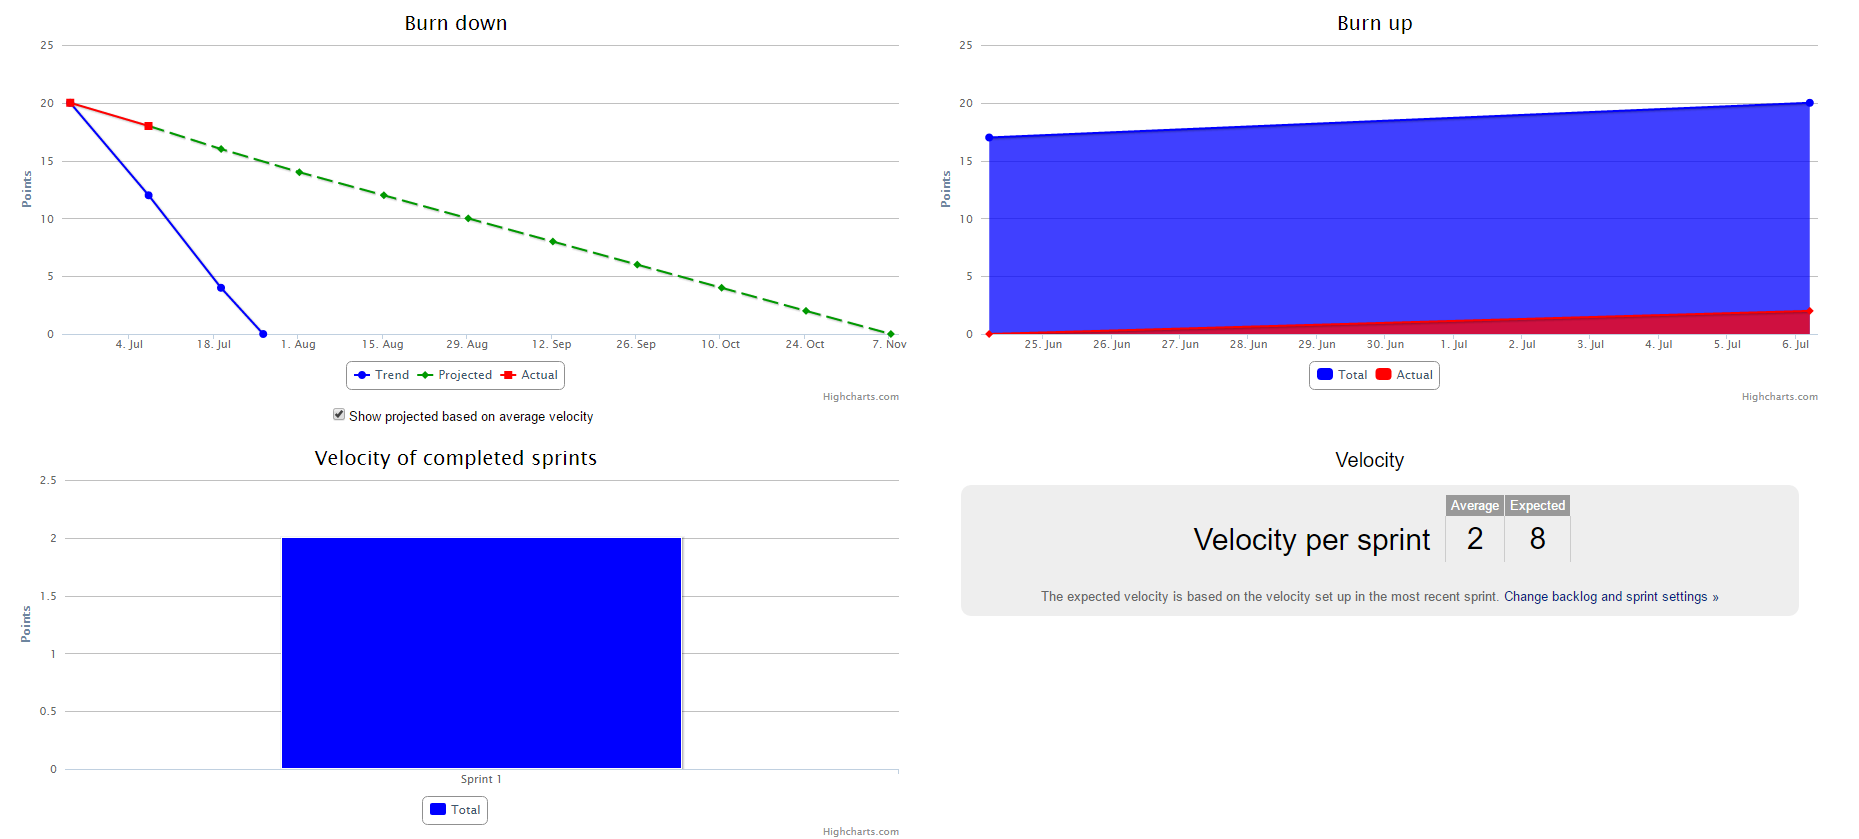
\includegraphics[width=0.9\textwidth]{images/Burndown_Sprint1}
    \caption{Example sprint burndown chart}
\end{figure}

\subsection{Sprint Retrospective}

At the end of each sprint the team discusses all of the sprint goals from the previous sprint, analyzes progress, and determines items that need to be changed or adjusted.

\subsection{Individual Status Reports}

Formal scrum meetings take place at the end of each class period with informal updates throughout the week via group messaging in GroupMe and emails/texting. 

\subsection{Engineering Notebooks}

Each individual team member is in charge of maintaining their own notebook, but ask for other team members to review as needed.

\subsection{Closeout Materials}

We will deliver the system as described in the mission statement and system overview to the University. The university will keep the Intel SR300 used by the project, and receive all related software, source code, and documentation in the form of a zip file. In addition, links will be provided to the online resources as described below. Other artifacts (Posters, supplemental materials, etc...) will also be provided to the university.

\subsubsection{System Prototype}

The system prototype will consist of open source software and an Intel SR300 camera. The university will retain the camera and software, with source code and documentation provided.

\subsubsection{Project Poster}

The team will collaborate to complete the poster and the end of Senior Design II.

\subsubsection{Source Code}

The source code will be maintained on GitHub, with each team member having access. The repository will be made public and the project will be made available as open source code for others to use and change.

\subsubsection{Source Code Documentation}

The source code documentation will be maintained with the source code in GitHub.

\subsubsection{Installation Scripts}

Instillation scripts will be maintained with the source code in GitHub.

\subsubsection{User Manual}

The user manual will help describe the use of the system to a user. It will be designed by the team and maintained in GitHub with the source code.